\tikzstyle{goal} = [draw, rectangle, minimum width=1cm, minimum height=2em, very thick, rounded corners=1mm]
\tikzstyle{ded}  = [-stealth,very thick]
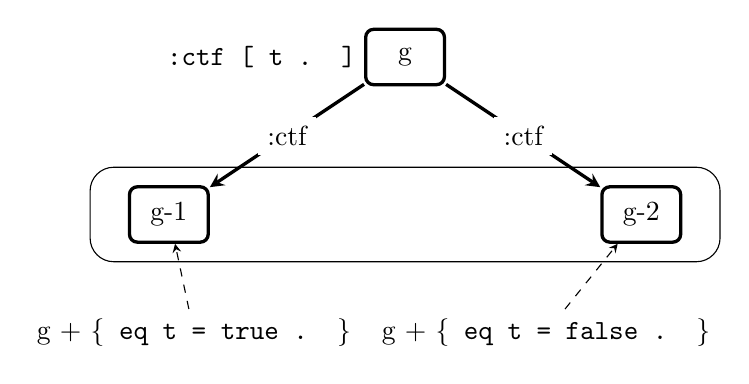
\begin{tikzpicture}[node distance=3cm]
  \node at (0,4) (g) [goal] {g};
  \node at (-3,2) (g-1)   [goal] {g-1};
  \node at (3,2) (g-2)   [goal] {g-2};
  \node [left of=g,node distance=0.5cm,anchor=east] {\texttt{:ctf [ t . ]}};
  \draw[rounded corners=3mm] (-4,1.4) rectangle (4,2.6);
  \path[ded] (g) edge node[fill=white] {:ctf} (g-1)
                 edge node[fill=white] {:ctf} (g-2) ;
  \node at (-4.8,0.5) (a) [anchor=west] {g + \texttt{\{ eq t = true . \}}} ;
  \node at  (4,0.5) (b) [anchor=east] {g + \texttt{\{ eq t = false . \}}} ;
  \path[-stealth,dashed] (a) edge (g-1) ;
  \path[-stealth,dashed] (b) edge (g-2) ;
%  \node at (-4.2,2) [anchor=east] {\texttt{:apply(RD)}} ;
\end{tikzpicture}
